\documentclass[border=5pt, multi, tikz]{standalone}

\definecolor{red}{rgb}{1,.5,.6}
\definecolor{blue}{rgb}{.7,.7,1}

\begin{document}
	
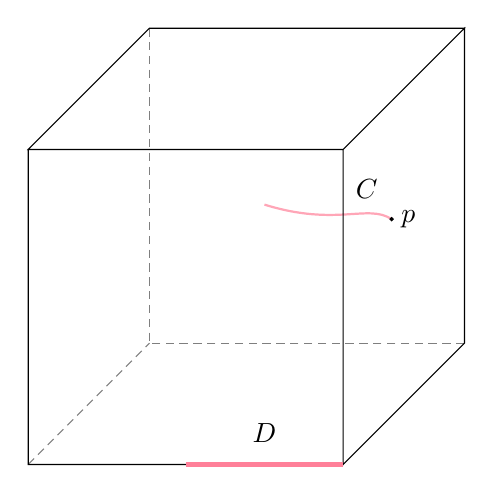
\begin{tikzpicture}
\coordinate (x) at (1,-.5,1);
\coordinate (c1) at (.7, -.3, 1);
\coordinate (c2) at (.3, -.6, 1);
\coordinate (z) at (-1,-.7,0);

\draw [opacity=.7, red, thick]
(x) .. controls (c1) and (c2) .. (z);

\node at (-1,-3.6,0){$D$};


\draw [every edge/.append style={draw=black, densely dashed, opacity=.5}]
(0,0,0) coordinate (o) --
++(-4,0,0) coordinate (a) --
++(0,-4,0) coordinate (b) edge
coordinate [pos=1] (g) ++(0,0,-4) -- ++(4,0,0) coordinate (c) -- cycle
(o) -- ++(0,0,-4) coordinate (d) -- ++(0,-4,0) coordinate (e) edge (g) -- (c) -- cycle
(o) -- (a) -- ++(0,0,-4) coordinate (f) edge (g) -- (d) -- cycle
;

\draw [ultra thick, red] (-2,-4,0) -- (0,-4,0);

\node at (.3,-.5,0){$C$};
\node[right] at (x){$p$};
\draw [fill] (x) circle [radius=0.02];
\end{tikzpicture}
\end{document}